A eletrônica embarcada do projeto tem como base 3 microcontroladores: o Arduino, o Raspberry Pi e o Galileo.

\begin{figure}[H]
	\centering
	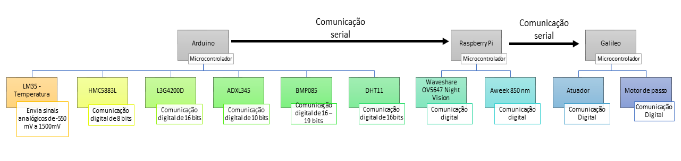
\includegraphics[width=0.8\textwidth]{figuras/eletronicaembarcadasum}
	\caption{Funcionamento geral da eletrônica embarcada no SUM.}
	\label{img:eletronicaembarcadasum}
\end{figure}

A Figura \ref{img:eletronicaembarcadasum} mostra o funcionamento geral da eletrônica embarcada do projeto. Os sensores que auxiliarão na estabilização do balão serão: LM35(Temperatura), HMC5883L(Bússola), L3G4200D(movimento), ADXL345(acelerometro), BMP085(pressão) e DHT11(umidade). Estes sensores estarão conectados em um Arduino UNO que, por sua vez, interpretará os dados dos sensores e mandará suas informações em série para o Raspberry Pi, que também estará conectado a um painel composto por vários LEDs para iluminação em infravermelho, o Aweek. Por fim, O Raspberry Pi mandará as informações para o microcontrolador Intel Galileo Gen 2, indicando se será necessária a estabilização da estrutura, de acordo com a interpretação feita pelo Arduino. Caso seja necessária a estabilização, o Galileo decidirá se ativará um motor de passo para realizar a estabilização através do trilho situado na payload, ou se ativará o atuador Reaction Wheel.

Raspberry Pi estará sendo utilizado também para transmitir as imagens em tempo real para a central. Ele receberá os dados da câmera, através do seu conector específico para câmera, e cada balão passará as informações para o balão mais próximo da central, a comunicação entre eles será sem fio montando uma rede intranet. O balão que esta recebendo tudo, transmitirá para a central através de um cabo de ethernet e o computador que recebe realizará todo o procedimento desejado com as imagens.

\subsection{Microcontroladores e microprocessadores}

Os microcontroladores e microprocessadores serão responsáveis por integrar todas as atividades do sistema, seja a aquisição, armazenamento, transmissão de dados, obtidos por sensores ou câmeras, conversão de dados analógicos em digitais ou o controle do sistema. Essas atividades exigirão determinados requisitos, de acordo com a sua aplicação. Logo, vê-se a necessidade de especificar os microprocessadores e microcontroladores responsáveis por cada setor. A iniciativa de usar um microcontrolador é baseada no fato deste possuir diversos periféricos e um processador embutidos em um único circuito integrado. Esta característica minimiza o tamanho físico do projeto e facilita a implementação de várias aplicações \cite{prado2009implementaccao}.  Contudo, as CPUs dos microcontroladores são menos poderosas do que as dos microprocessadores, suas instruções, geralmente, se limitam às instruções mais simples, sua frequência de clock é menor e seu espaço de memória endereçável costuma ser menor \cite{rucinski}.

Em condições desfavoráveis, como por exemplo um fluxo de ar inesperado, a rápida estabilização do balão se mostra essencial para a captação das imagens, visando sua qualidade. O setor voltado para o controle e estabilização exigirá uma frequência de clock muito alta, pois esta deverá ser realizada rapidamente. Portanto, essa função será desempenhada pelo Intel Galileo Gen 2, pois este admite frequências de clock de até 400 MHz. Além disso, é compatível com os shields feitos para Arduino UNO e com o seu ambiente de desenvolvimento (IDE), o que torna sua codificação mais prática.

Para os setores de armazenamento e transmissão de imagens das câmeras, o Raspberry PI 2 foi considerado o ideal, dado sua eficiência em termos de processamento de dados. Outra vantagem de se utilizar o Raspberry é a sua compatibilidade com a linguagem Python, o que facilitará o desenvolvimento do algoritmo responsável pela compressão de vídeo.

Para o setor voltado para a captação de dados dos sensores, decidiu-se que o ideal seria utilizar o Arduino UNO, visto que este possui grande compatibilidade com os shields escolhidos, além de uma quantidade razoável de portas disponíveis.

As especificações dos microcontroladores estão relacionadas na tabela \ref{table:microprocessadores}:

\begin{table}[H]
\centering
\begin{tabular}{p{3cm}|p{3cm}|p{3cm}|p{3cm}|}
\cline{2-4}
 & Intel Galileo Gen 2 & Raspberry PI 2 & Arduino UNO \\ \hline
\multicolumn{1}{|l|}{Microcontrolador} & \multicolumn{1}{c|}{-} & \multicolumn{1}{c|}{-} & ATmega328 \\ \hline
\multicolumn{1}{|l|}{Processador} & SoC Quark X1000 - 32 bits & Broadcom BCM2836 SoC & \multicolumn{1}{c|}{-} \\ \hline
\multicolumn{1}{|l|}{Arquitetura} & x86 & Quad-core ARM Cortex-A7 & \multicolumn{1}{c|}{-} \\ \hline
\multicolumn{1}{|l|}{Memória} & DDR3 de 256 MB, SRAM embarcada de 512 KB, NOR Flash de 8 MB e EEPROM padrão de 8 KB on-board & 1 GB de RAM & 32K (0.5 usado pelo bootloader) \\ \hline
\multicolumn{1}{|l|}{Clock} & 400 MHz & 900 MHz & 16MHz \\ \hline
\multicolumn{1}{|l|}{GPU} & \multicolumn{1}{c|}{-} & VídeoCore IV & \multicolumn{1}{c|}{-} \\ \hline
\multicolumn{1}{|l|}{Portas analógicas} & 6 & \multicolumn{1}{c|}{-} & 6 \\ \hline
\multicolumn{1}{|l|}{Portas digitais} & 14 & 26 (GPIO) & 14 \\ \hline
\multicolumn{1}{|l|}{Portas PWM} & 6 (12-bit) & \multicolumn{1}{c|}{-} & 6 \\ \hline
\multicolumn{1}{|l|}{Tensão de operação} & 12 V & 5 V & 5 V \\ \hline
\multicolumn{1}{|l|}{Corrente máxima} & 2 A & 1 A & 40 mA \\ \hline
\multicolumn{1}{|l|}{Alimentação} & 7 - 15 V & 5 V & 7 -12 Vdc \\ \hline
\multicolumn{1}{|l|}{Interface Ethernet} & 10/100 Mbps & 10/100 Mbps & \multicolumn{1}{c|}{-} \\ \hline
\multicolumn{1}{|l|}{Saída de vídeo e Áudio} & \multicolumn{1}{c|}{-} & HDMI e Av & \multicolumn{1}{c|}{-} \\ \hline
\end{tabular}
\caption[Especificações dos microcontroladores]{Especificações dos Microcontroladores~\cite{intelGalileo},\\\cite{rsppi}, \cite{arduino}}
\label{table:microprocessadores}
\end{table}

\subsection{Sensores}

Para os sensores utilizados nesse projeto que já possuem internamente um conversor de sinal analógico para digital e também um filtro para reduzir ruídos, o funcionamento é basicamente coletar a informação desejada, fazer a conversão de dados para digital, logo após realiza a filtragem e realizada a filtragem esses dados são passados para uma memória e para um bloco onde vai controlar essas informações no sistema de comunicação I2C.

O sistema de comunicação I2C possibilita utilizar, em um mesmo sistema, componentes de tecnologias construtivas diferentes sem que haja incompatibilidade e nem conflitos na comunicação.

A transmissão da informação entre os dispositivos é feita através de dois fios, serial data DAS e serial clock SCL.

\begin{figure}[H]
	\centering
	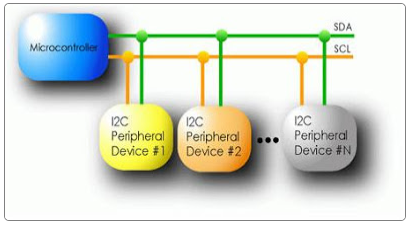
\includegraphics[width=0.8\textwidth]{figuras/1}
	\caption{Exemplo de funcionamento da comunicação I2C \cite{microcontrolandos}.}
	\label{img:funcionamentoI2c}
\end{figure}

Os dispositivos ligados em Inter IC possuem um endereço fixo (cada componente recebe um endereço específico), e podemos configurá-los para receber ou transmitir dados; dessa maneira eles podem ser classificados de várias formas, como: mestres (MASTER), escravos (SLAVE), entre outras.

Uma das vantagens do padrão I2C é que ele não fixa a velocidade de transmissão (freqüência), pois ela será determinada pelo circuito MASTER (transmissão do SCL).

O Diagrama de funcionamento dos sensores são demonstrados nas figuras de \ref{img:acelerometro} à \ref{img:sensorumidade}.

\begin{itemize}
  \item Acelerômetro
  \begin{figure}[H]
    \centering
    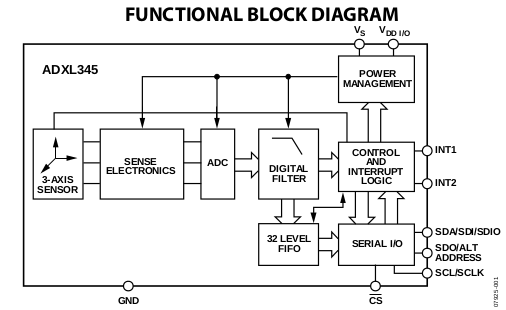
\includegraphics[width=0.8\textwidth]{figuras/2}
    \caption{Diagrama funcional acelerômetro ADXL345 \cite{acelerometro}.}
    \label{img:acelerometro}
  \end{figure}
  \item Barômetro
  \begin{figure}[H]
    \centering
    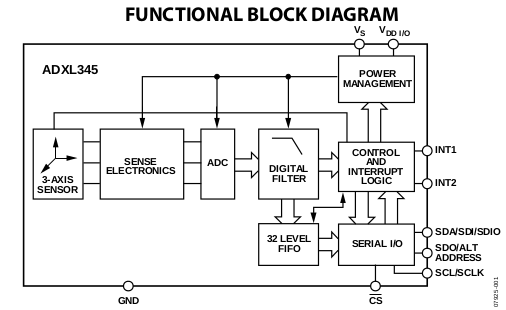
\includegraphics[width=0.8\textwidth]{figuras/2}
    \caption{Diagrama funcional Barômetro BMP085 \cite{barometro}.}
    \label{img:barometro}
  \end{figure}
  \item Giroscópio
  \begin{figure}[H]
    \centering
    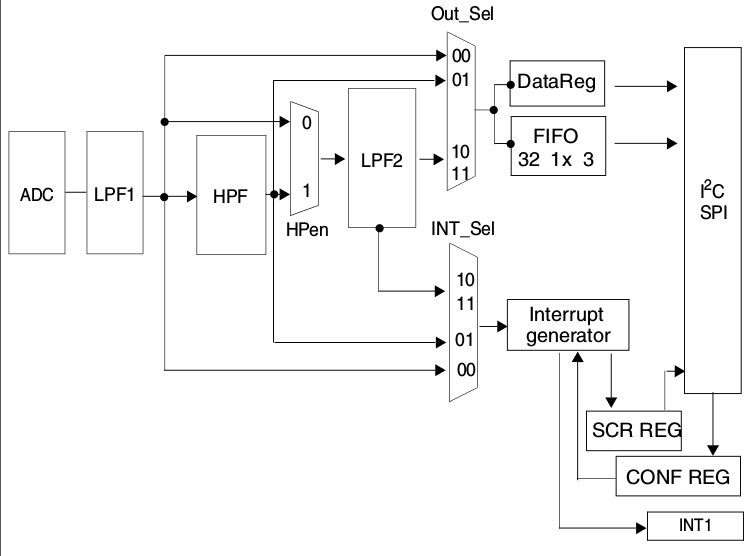
\includegraphics[width=0.8\textwidth]{figuras/4}
    \caption{Diagrama Funcional Giroscópio L3G4200D \cite{giroscopio}.}
    \label{img:giroscopio}
  \end{figure}
  \item Magnetômetro
  \begin{figure}[H]
    \centering
    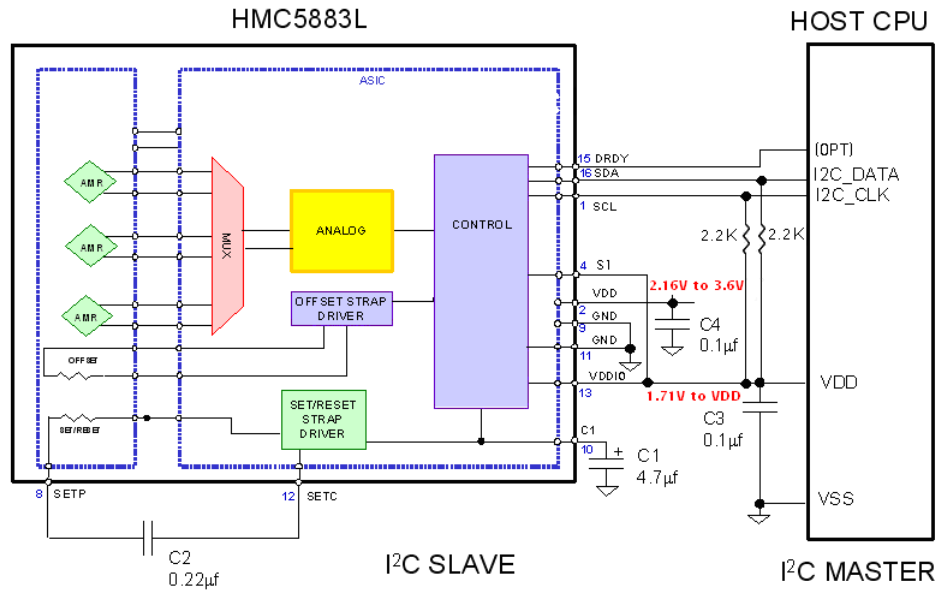
\includegraphics[width=0.8\textwidth]{figuras/6}
    \caption{Diagrama funcional magnetômetro HMC5883L \cite{magnetometro}.}
    \label{img:magnetometro}
  \end{figure}
  \item Sensor de umidade
  \begin{figure}[H]
    \centering
    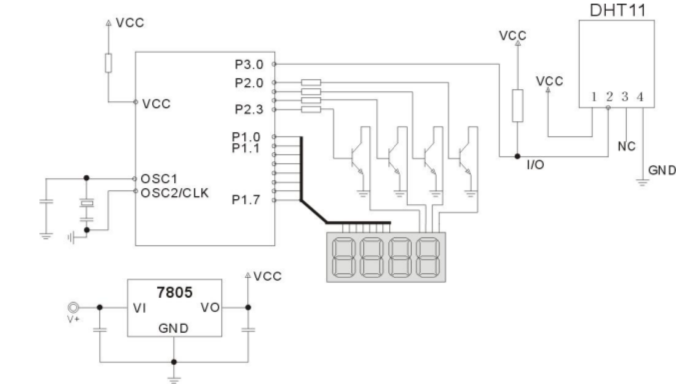
\includegraphics[width=0.8\textwidth]{figuras/5}
    \caption{Diagrama funcional sensor de umidade \cite{sensorhumidade}.}
    \label{img:sensorumidade}
  \end{figure}
\end{itemize}

A conversão Analógico/Digital será feita internamente nos sensores, como foi mostrado em seus respectivos diagramas funcionais, o que significa que fornecerão valores digitais em suas saídas, que estarão conectadas a um microcontrolador.

Geralmente, os microcontroladores processam dados obtidos por sensores e na sua saída são encontrados valores analógicos, logo é necessário transformá-los em valores digitais. Então, para executar essa atividade, é preciso do conversor A/D, que inter-faceiam os dispositivos de medidas e o microcontrolador.

Nesses conversores, quanto maior o número bits de saída, melhor ele será. Por exemplo, um conversor que tem uma saída de quatro bits possui dezesseis degraus de indicação, ou seja, pode definir uma escala de dezesseis valores diferentes.

\begin{figure}[H]
  \centering
  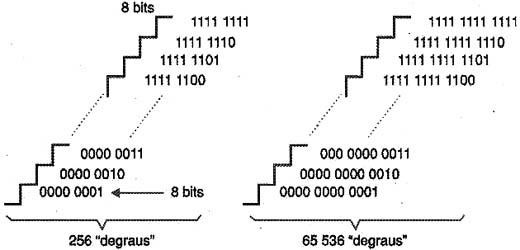
\includegraphics[width=0.8\textwidth]{figuras/ADC}
  \caption{Ilustração da escala de bits.}
  \label{img:escaladebits}
\end{figure}

Se o circuito converte sinais na faixa de 0V a 1V, é preciso ter cuidado para que os sensores usados trabalhem nessa faixa. Um amplificador operacional pode ter um ganho programado para evitar esses problemas. Então, as saídas terão um número n de pinos nas quais as saídas nos níveis lógicos 0 ou 1 são obtidos conforme a tensão de entrada \cite{conversoresad}.

\subsection{Sistemas de câmeras}

Cada balão portará 1 câmera direcionada para a região em que se efetuará a monitoração. A câmera escolhida foi a Waveshare OV5647 Night Vision, com as seguintes especificações técnicas:

\begin{itemize}
	\item 5MP.
	\item Vídeo: 1080 p.
	\item Abertura (F): 2.9
	\item Distância Focal: 3.29 mm.
	\item Diagonal: 72.4 mm.
	\item Dimensões: 25 mm x 24 mm x 6 mm.
	\item Suporta até 2 LEDs infra-vermelhos.
	\item Massa: $1,7\times 10^{-2}$ kg.
	\item Preço: U\$30.99.
\end{itemize}

\begin{figure}[H]
  \centering
  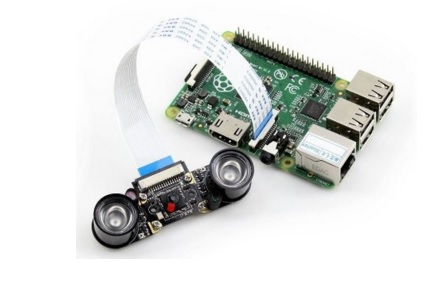
\includegraphics[width=0.8\textwidth]{figuras/RSP}
  \caption[Waveshare OV5647 Night Vision em destaque]{Waveshare OV5647 Night Vision em destaque~\cite{amazon1}}
  \label{img:Waveshare}
\end{figure}

\begin{figure}[H]
  \centering
  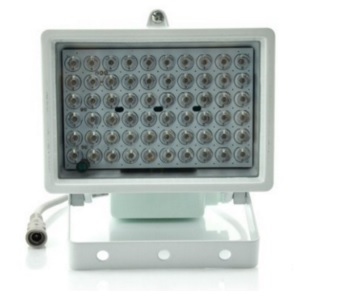
\includegraphics[width=0.8\textwidth]{figuras/Painel}
  \caption[Painel infra-vermelho]{Painel infra-vermelho~\cite{amazon2}}
  \label{img:painel}
\end{figure}

A câmera foi escolhida dada a sua alta resolução, fácil interface com o Raspberry PI, o sensor ser adequado para ser utilizado com o infravermelho para filmagens noturnas. Além disso, possui dimensões pequenas. O fabricante não informa o alcance do infravermelho para filmagens noturnas, dessa forma faz-se necessária a utilização conjunta com  câmera de um painél infravermelho externo. O painel escolhido é denominado: Aweek 850 nm, 60 LEDs IR com especificações:

\begin{itemize}
	\item Comprimento de onda: 850 nm.
	\item Consumo: 12 W.
	\item Tensão de operação: 12 VDC.
	\item Alcance: 60 m.
	\item Massa: 0.5 kg.
	\item Preço: U\$27.88.
\end{itemize}

As câmeras serão fixadas ao balão, e por estarem acondicionadas em seus respectivos invólucros (caixas de proteção) deverão continuar operando perfeitamente sob temperatura ambiente
entre 0 e 40$^{\circ}$C e umidade relativa do ar de até 90\%.

\subsection{Estabilização da carga útil}

Embora que a princípio o balão trabalhará com altitude fixa, este tem o grau de liberdade para mudar de orientação em torno dos eixos ZB, YB e XB (considera-se o sistema de referência Body Axes), figura \ref{img:eixosreferencia}. O sistema de referência nos eixos do corpo tem origem geralmente no centro de massa, e utilizada para referenciar aeronaves, neste caso será aplicado à payload do balão. Estas mudanças de orientação ocasionarão a rotações involuntárias de câmeras embarcadas no balão, dessa forma faz-se necessária a estabilização do movimento.

\begin{figure}[H]
  \centering
  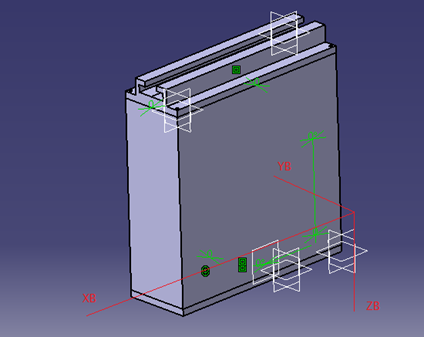
\includegraphics[width=0.8\textwidth]{figuras/estrutura}
  \caption{Eixos de referência em destaque.}
  \label{img:eixosreferencia}
\end{figure}

Tal movimento de rotação pode ser induzido pelas forças aerodinâmicas que agem no balão quando o fluxo de ar faz-se presente. O sistema de controle que seria capaz de estabilizar o sistema frente a uma perturbação seria classificado como de malha fechada, isso significa que um conjunto de sensores inerciais (acelerômetro, giroscópio) deve ser empregado para além de detectar a perturbação, verificar se o sistema de controle está sendo efetivo. Dessa forma o sistema de controle de malha fechada verifica se a saída condiz com as especificações de estabilidade do sistema, para se ter certeza de que a estabilização está sendo feita. O sistema de controle atuaria de forma intermitente enquanto a estabilização não fosse bem sucedida. Para fins de viabilidade, o sistema de controle empregado deve ser capaz de estabilizar a payload (setor de equipamentos embarcados) rapidamente, para se ter qualidade nas imagens geradas pela câmera.

Um provável atuador para o eixo ZB, ou seja, mecanismo capaz de efetuar a estabilização seria um Reaction Wheel. Um Reaction Wheel é um dispositivo frequentemente utilizado para o controle de atitude de satélites, consiste de um disco massivo acoplado a um eixo giratório. O princípio que o dispositivo usa para efetuar a estabilização é o momento de inércia do disco, dependendo da interpretação do algoritmo de controle das leituras dos sensores, sua rotação é ativada com velocidade e sentido determinados, executando-se a estabilização (anula a rotação da payload do balão no eixo). Tal atuador se encontrará no interior da payload.

Para a estabilização do eixo YB pode ser utilizado um trilho para mover a posição da bexiga, e dessa forma alterar o ângulo de pitch, de forma a nivelar o plano seccional horizontal da payload com o solo. Tal trilho está indicado na estrutura conceitual da payload, figura \ref{img:trilhoestrutura}.

\begin{figure}[H]
  \centering
  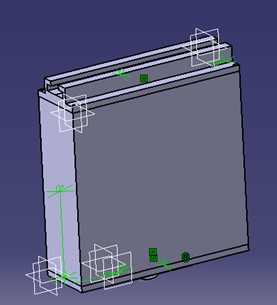
\includegraphics[width=0.8\textwidth]{figuras/e2}
  \caption{Trilho em destaque na estrutura conceitual da payload.}
  \label{img:trilhoestrutura}
\end{figure}

No caso o eixo XB, a estabilização pode ser feita através da variação da altitude do balão em intervalos de distância pré-definidos. Essa variação da altitude pode ser feita através da retração e liberação do cabo na carretilha em solo. A instabilidade no eixo ZB não afetará significativamente a qualidade da imagem, desde que a estabilização nos outros dois eixos seja efetiva.

Uma provável automação efetuada pelo balão será a avaliação de sua própria segurança. Por meio de sensores de tensão no cabo (dinamômetro) preso na estrutura da figura \label{img:caboancoragem}, se esta aumentar acima de um nível critico, este será automaticamente recolhido por meio do rotor motorizado em solo, e a estação de solo será informada. Assim que o sensor em solo sinalizar normalidade na velocidade do vento este será novamente elevado.

\begin{figure}[H]
  \centering
  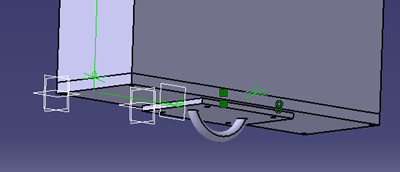
\includegraphics[width=0.8\textwidth]{figuras/e3}
  \caption{Conexão com cabo de ancoragem em destaque.}
  \label{img:caboancoragem}
\end{figure}


Mais uma automação essencial será a sua elevação e retração automática para o período de monitoração determinada.

O funcionamento completo do sistema de estabilização se dará da seguinte forma: quando o sistema aéreo é ativado, ocorrerá a auto-orientação da carga útil (payload). Tal auto-orientação buscará direcionar a câmera para uma dada região pré determinada. Posteriormente, qualquer perturbação que gere alteração da atitude (orientação) da carga útil deverá ser corrigida pelos atuadores, isto é, Reaction Wheel e trilho.

O reaction wheel escolhido é o da companhia Clyde Space possuindo as seguintes especificações técnicas:

\begin{table}[H]
	\centering
	\begin{tabular}{|l|c|c|l|}
	\hline
	\rowcolor[HTML]{C0C0C0}
	\textbf{Característica}          & \textbf{Valor} & \textbf{Unidades} & \textbf{Notas}        \\ \hline
	Máxima velocidade volante        & 66500          & rpm               & @28 V                 \\ \hline
	Torque máximo à 6500 rpm         & 26             & mNm               & @28 V                 \\ \hline
	Torque máximo até 2500 rpm       & 40             & mNm               & @28 V                 \\ \hline
	Faixa de temperatura em operação & -20 a 50       & ºC                & \multicolumn{1}{c}{-} \\ \hline
	Faixa de temperatura em repouso  & -30 a 60       & ºC                & \multicolumn{1}{c}{-} \\ \hline
	Consumo quando inativo           & 1.5            & W                 & @28 V                 \\ \hline
	Consumo sem carga                & \textless 12   & W                 & @28 V                 \\ \hline
	Consumo em torque máximo         & \textless 28   & W                 & @28 V                 \\ \hline
	Inércia do disco                 & 0.001766969    & kg*$m^{2}$        & \multicolumn{1}{c}{-} \\ \hline
	Massa total do dispositivo       & 1.5            & Kg                & \multicolumn{1}{c}{-} \\ \hline
	\end{tabular}
	\caption[Especificação do Reaction Wheel]{Especificação do Reaction Wheel~\cite{clyde}}
	\label{tab:reactionWheel}
\end{table}

Para fazer a bexiga se locomover no trilho, faz-se necessária a utilização de um motor de passo. O motor escolhido foi o de modelo AK23/R100F6FN1.8-G10-LINIX com caixa de redução, devido ao torque, dimensões e consumo.

\begin{figure}[H]
  \centering
  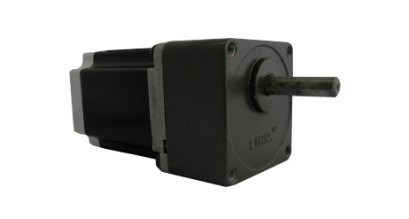
\includegraphics[width=0.8\textwidth]{figuras/M}
  \caption[Motor de Passo AK23/R100F6FN1.8-G10-LINIX]{Motor de Passo AK23/R100F6FN1.8-G10-LINIX~\cite{robocore}}
  \label{img:motorpasso}
\end{figure}

Dados técnicos do motor:

\begin{itemize}
	\item Tensão: 2.4 VDC.
	\item Corrente: 3 A.
	\item NEMA: 23.
	\item Folga: a folga do redutor é de 30 arcminutos (0.5 graus).
	\item Marca: LINIX.
	\item Preço: R\$359.00.
\end{itemize}

Para ser controlado, esse motor requer um driver, o modelo escolhido, por se adequar as especificações técnicas do motor foi o SparkFun AutoDriver - Stepper Motor Driver com as seguintes especificações~\cite{pololu}:

\begin{itemize}
	\item Detecção de superaquecimento.
	\item Deterção de excesso de corrente.
	\item Controlado por SPI.
	\item ADC de 5 bits.
	\item Faixa de tensão: 8 - 45 V.
	\item Corrente suportada: 3 A.
	\item Preço: U\$34.95.
\end{itemize}
